%Use the compiler XeLaTex for the cover!!

\documentclass[12pt]{article}
% load the necessary packages
\usepackage[spanish]{babel}
%\usepackage[english]{babel}
\usepackage[latin1]{inputenc}
\usepackage[paperheight=26.67cm,paperwidth=36.15cm,margin={0pt,0pt},bindingoffset=-6mm]{geometry}
\usepackage[dvipsnames,prologue,table]{pstricks}
\usepackage{pst-all}
\usepackage{pst-grad}
\usepackage{graphicx}
\usepackage{rotating}
\usepackage{color}
\usepackage{calc}
%\usepackage[ISBN=978-80-85955-35-4]{ean13isbn}
%\EANisbn[SC4]

\usepackage{fp}

\makeatletter

% Deep Carrot Orange
\definecolor{Maroon}{rgb}{0.91, 0.41, 0.17}

\FPset{margenancho}{0.32}
\FPset{margenalto}{0.335}
\FPset{alto}{26}
\FPset{ancho}{16.82}
\FPset{lomo}{1.867}
\FPset{iniciolomo}{17.14}
\FPset{anchobandamaroonportada}{2.3}
\FPset{anchobandawhitecontraportada}{2.7}
\FPset{anchobanda}{2}
\FPset{widthUGR}{5.446} %5.046
\FPset{widthETSIIT}{1.45}
\FPset{widthoATC}{5.477}
\FPset{altoescudos}{1}
\FPset{cuadrofotobiografia}{7.8}

\FPeval{altocompleto}{\margenalto + \alto + \margenalto}
\FPeval{anchocompleto}{\margenancho + \ancho + \lomo + \ancho + \margenancho}
\FPeval{inicioportada}{\margenancho + \ancho + \lomo}
\FPeval{contraportada}{\margenancho}
\FPeval{bandamaroonportada}{\inicioportada + \anchobandamaroonportada}
\FPeval{altomenosmargen}{\altocompleto - \margenalto}
\FPeval{anchomenosmargen}{\anchocompleto - \margenancho}

\FPeval{centrolomo}{(\iniciolomo + \inicioportada)/ 2}
\FPeval{centrolomosuperior}{\centrolomo + 0.3}
\FPeval{centrolomoinferior}{\centrolomo -0.3}

\FPeval{financhobandacontraportada}{\anchobandawhitecontraportada + \anchobanda}
\FPeval{letraswhitebandacontraportada}{\financhobandacontraportada - 0.2}
\FPeval{letrasmaroonbandacontraportada}{\financhobandacontraportada -1.15}

\FPeval{financhobandaportada}{\bandamaroonportada}
\FPeval{letraswhitebandaportada}{\financhobandaportada - 1.57}
\FPeval{letrasmaroonbandaportada}{\financhobandaportada - 0.45}

\FPeval{mitadblancaportada}{(\anchocompleto + \financhobandaportada) / 2 }
\FPeval{mitadportadadesplazada}{\mitadblancaportada + 1}

\FPeval{mitadmarooncontraportada}{(\financhobandacontraportada + \iniciolomo) / 2 }
\FPeval{mitadcontraportadadesplazada}{\mitadmarooncontraportada + 1}

\FPeval{fotobiografia}{\cuadrofotobiografia}
\FPeval{fincuadrofotobiografia}{\cuadrofotobiografia + 1.2}
\FPeval{textobiografia}{\fincuadrofotobiografia + 1.1}

\FPeval{anchoUGR}{\iniciolomo - 0.2}
\FPeval{anchoETSIIT}{\anchoUGR - \widthUGR - 0.2}
\FPeval{anchoATC}{\anchoETSIIT - \widthETSIIT - 0.5}

% begin the document and suppress page numbers
\begin{document}
%\pagecolor{Maroon}
\pagestyle{empty}
% create the box with the front cover picture
\newsavebox\IBox
\sbox\IBox{
\includegraphics[width=14cm]{cover_gfx/bordesLogoUGRcover.eps}}

\newsavebox\UGRBox
\sbox\UGRBox{
\includegraphics[height=1.7cm]{cover_gfx/logougr.eps}}

\newsavebox\ETSIITBox
\sbox\ETSIITBox{
\includegraphics[height=1.7cm]{cover_gfx/logoetsiit.eps}}

\newsavebox\ATCBox
\sbox\ATCBox{
\includegraphics[height=1.7cm]{cover_gfx/logoatc.eps}}


% set up the picture environment
\psset{unit=1cm}

\begin{pspicture}(0,0)(\anchocompleto,\altocompleto)
\psframe[fillstyle=solid,fillcolor=Maroon,linewidth=0pt,linecolor=Maroon](0,0)(\bandamaroonportada,\altocompleto)

\newfont{\TituloPrincipalFont}{pncb scaled 4500}%{eurb10 scaled 7000}%
\newfont{\TituloSegundoFont}{pncb scaled 7805}%{pncb scaled 4500}%{eurb10 scaled 7000}%

% place the front cover picture
\rput[c]{45}(33cm,3cm){\usebox\IBox}

% Letras montadas sobre banda Maroon
\rput[lt]{90}(\letraswhitebandaportada,3.7){\TituloPrincipalFont \color{white}{Universidad de Granada}}
\rput[lt]{90}(\letrasmaroonbandaportada,3.7){\TituloSegundoFont \color{Maroon}{Tesis Doctoral}}

% put the text on the front cover
\newsavebox\Titlebox
\sbox\Titlebox{\begin{minipage}{11cm}
\centering\textcolor{black}{\textsc{\Large DARP: A new routing algorithm for large communication infrastructures}}
\end{minipage}}

\rput[ct](\mitadportadadesplazada,20){\usebox\Titlebox}
\rput[ct](\mitadportadadesplazada,19){\color{black}{\textsc{\normalsize Francisco Jos\'e Est\'evez Ortiz}}}
\rput[c](\mitadblancaportada,25.5){\textsc{\footnotesize Departamento de Arquitectura y Tecnolog\'{\i}a de Computadores}}
\rput[c](\mitadblancaportada,25.2){\textsc{\scriptsize Escuela T�cnica Superior de Ingenier�as Inform�tica y de Telecomunicaci�n}}
\rput[c](\mitadblancaportada,24.9){\textsc{\scriptsize Universidad de Granada}}


% put the text on the spine (note the rotation over 270 degrees)

\rput[c](\centrolomo,23){ \begin{turn}{-90}
{
\color{white} {\Large Tesis Doctoral}
} \end{turn} }

\rput[c](\centrolomosuperior,13){ \begin{turn}{-90}
{
\color{white} \textsc{\small DARP: A new routing algorithm for large communication infrastructures}
} \end{turn} }

\rput[c](\centrolomoinferior,13){ \begin{turn}{-90}
{
\color{white} \textsc{\footnotesize Francisco Jos\'e Est\'evez Ortiz}
} \end{turn} }

\rput[c](\centrolomo,2.5){\color{white}\textbf{2016}}

% Then we close all open environments
% 
% %%%%%%%%%%%%%%%%%%%%%%%%%%%%%%%%%%

\psframe[fillstyle=solid,fillcolor=white,linewidth=0pt,linecolor=white](\anchobandawhitecontraportada,0)(\financhobandacontraportada,\altocompleto)
\rput[rb]{270}(\letraswhitebandacontraportada,3.7){\TituloSegundoFont \color{white}{Tesis Doctoral}}
\rput[rb]{270}(\letrasmaroonbandacontraportada,3.7){\TituloPrincipalFont \color{Maroon}{Universidad de Granada}}

\rput[rb](\anchoUGR,\altoescudos){\usebox\UGRBox}
\rput[rb](\anchoETSIIT,\altoescudos){\usebox\ETSIITBox}
\rput[rb](\anchoATC,\altoescudos){\usebox\ATCBox}

\newsavebox\Authorbox
\sbox\Authorbox{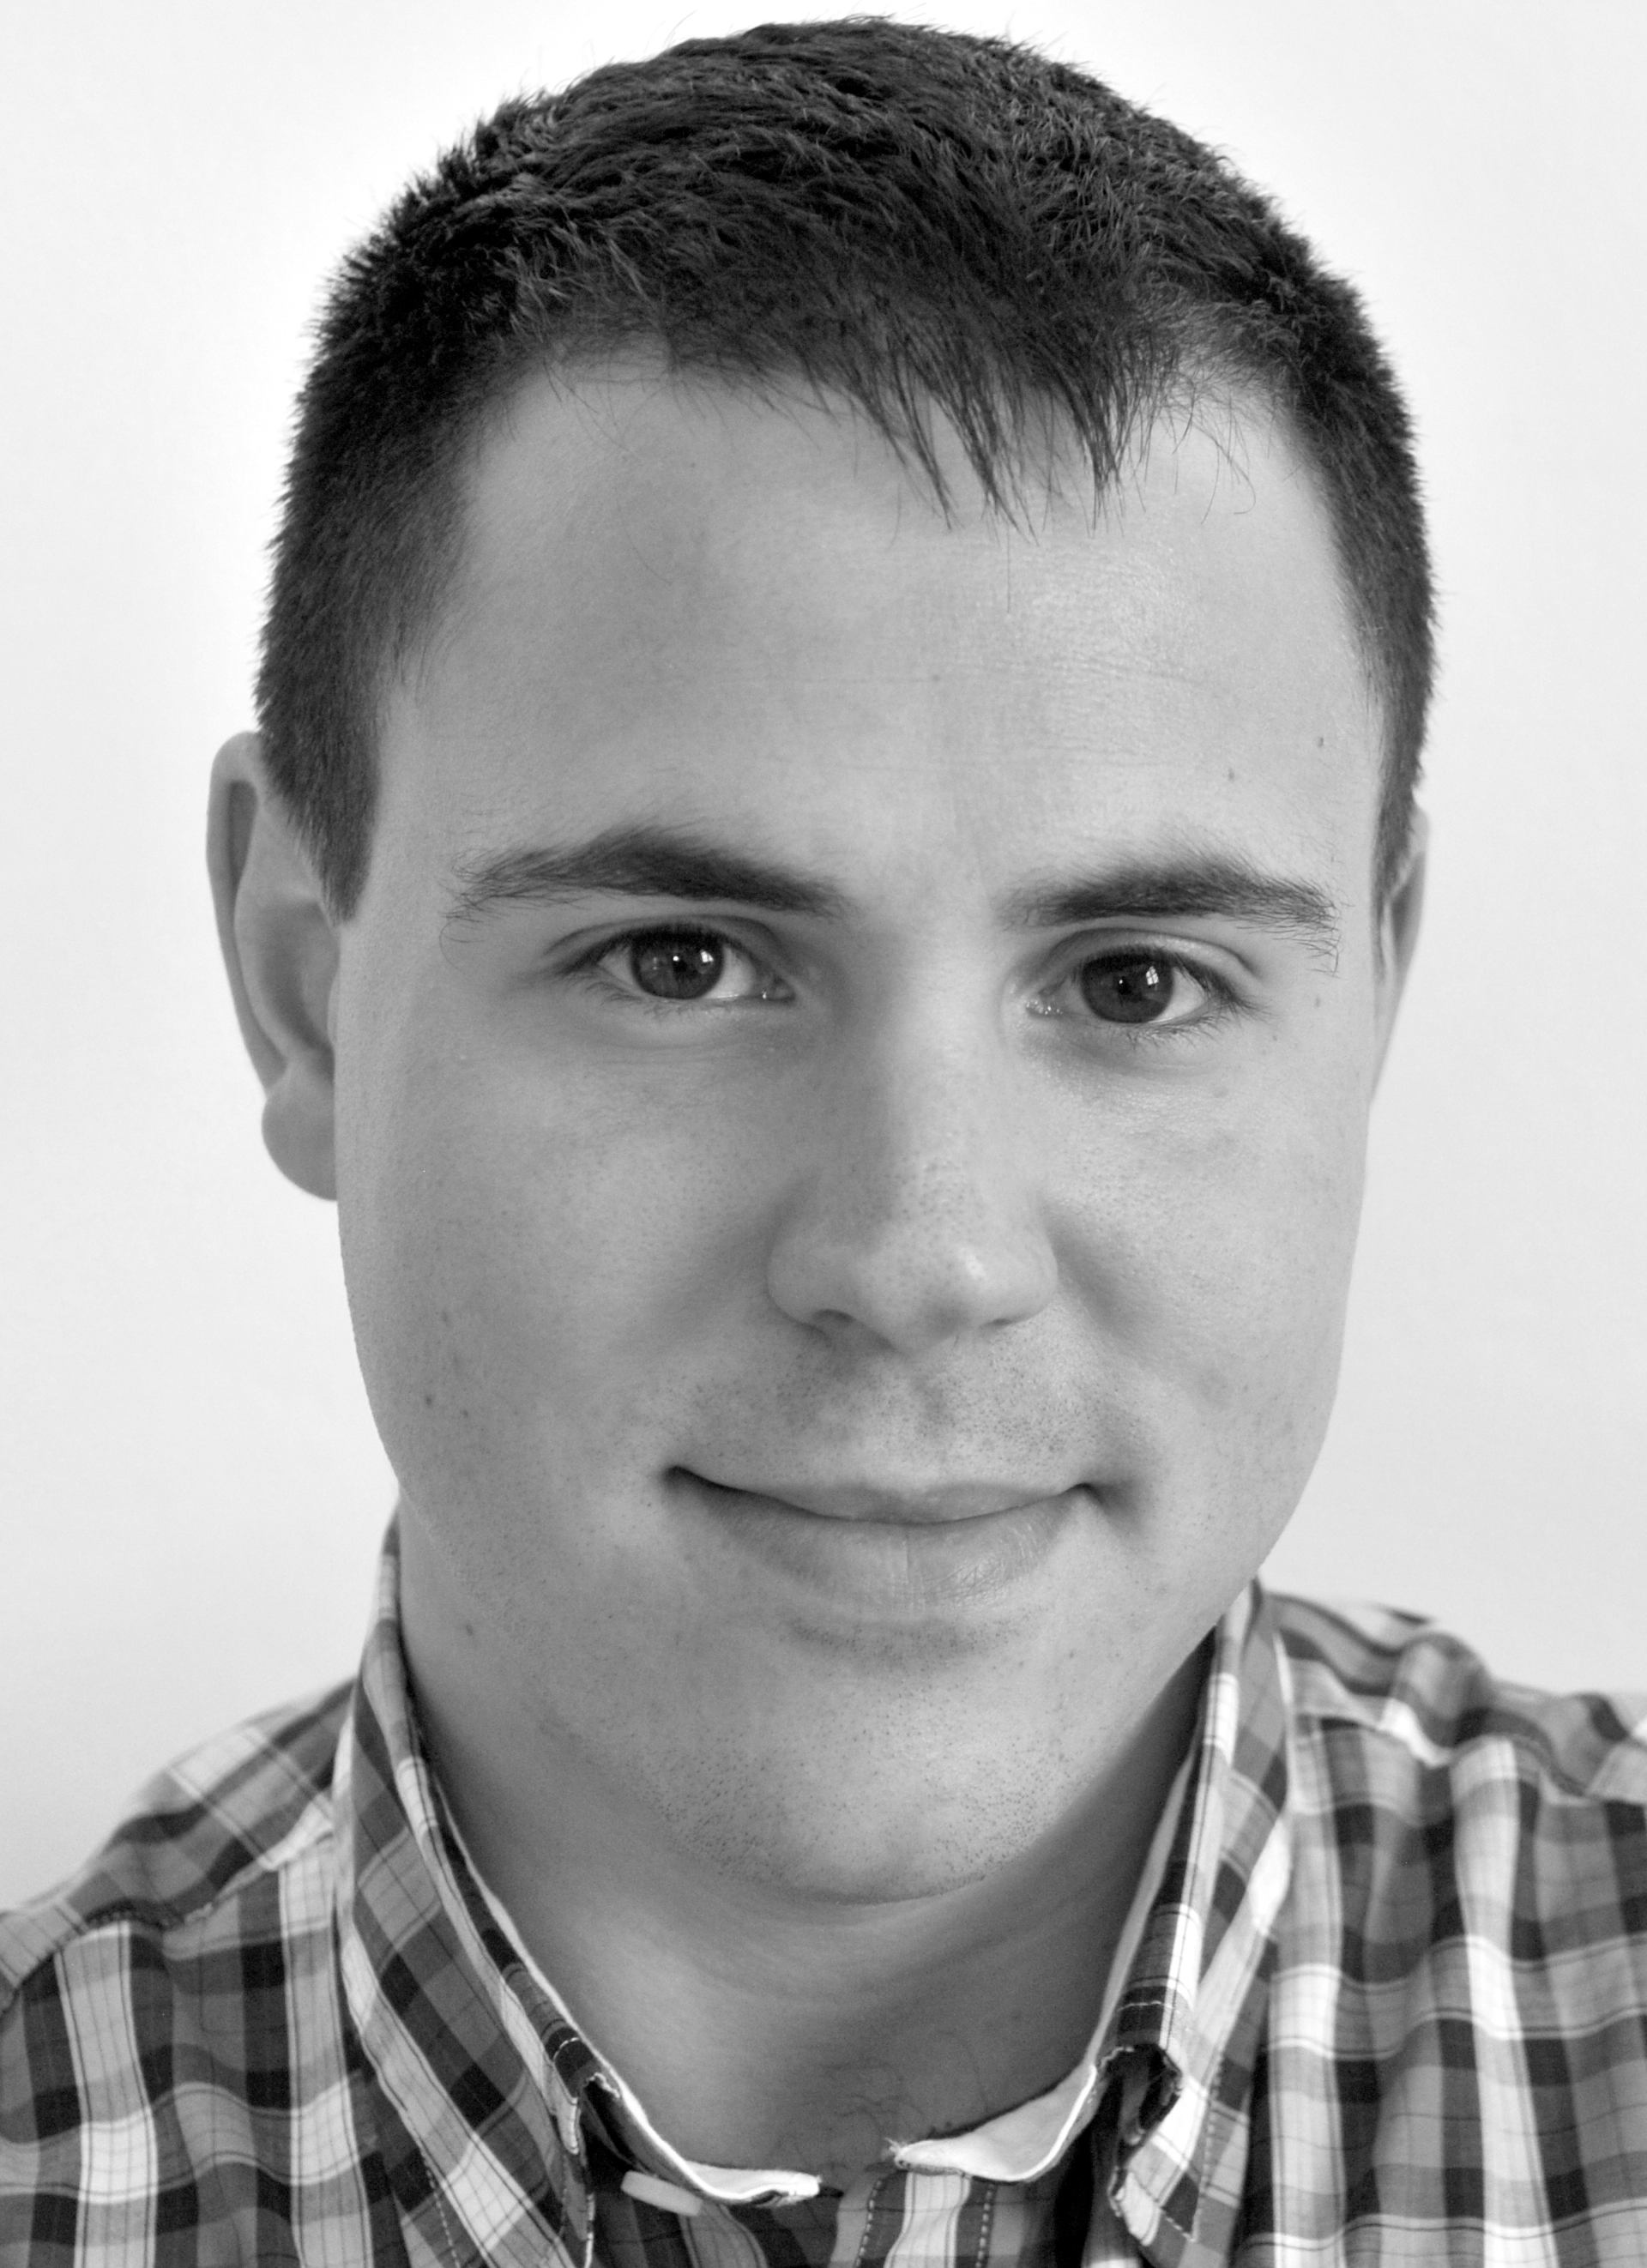
\includegraphics[width=2cm]{cover_gfx/fcoestevez_grayscale.png}}

% A white box in which place the photo
%\psframe[fillstyle=solid,fillcolor=white](\cuadrofotobiografia,22.6)(\fincuadrofotobiografia,23.4)
% now place the picture
\rput[lt](\fotobiografia,23.5){\usebox\Authorbox}
% create a savebx for the biography. The width has been adjusted so
% that the right margin matches with that of the book blurb
\newsavebox\Biobox
\sbox\Biobox{\begin{minipage}{6cm}
\textcolor{white}{\scriptsize \textsc{Francisco Jos\'e Est\'evez Ortiz} es Diplomado y Licenciado en Inform\'atica por la Universidad de C\'ordoba en 2008 y 2010 respectivamente. En 2011 obtuvo su Maestr\'ia en Arquitectura de Computadores y Redes por la Universidad de Granada. En 2011 comenz\'o su andadura profesional como investigador en la empresa CILAB, para posteriormente, en 2012, pasar a formar parte de Zodiac Aerospace. Desde el 2013 trabaja como investigador en el Laboratorio de Semiconductores y Sistemas bus de la Universidad de Ciencias Aplicadas de Muenster, Alemania. Su e-mail de contacto es: \texttt{fjestevez@ieee.org}}
\end{minipage}}
% and put it where it belongs
\rput[tl](\textobiografia,23.5){\usebox\Biobox}

% Create a Box containing the text for the back cover
\newsavebox\Blurbbox
\sbox\Blurbbox{\begin{minipage}{8.5cm}
\textcolor{white}{{\huge L}\footnotesize\textsc{a} presente Tesis Doctoral presenta un nuevo protocolo de enrutamiento (\textsc{DARP}) orientado a la gesti\'on de la infraestructura de las Ciudades Inteligentes. Dicho protocolo est\'a basado en la selecci\'on din\'amica del rol de los nodos y la creaci\'on de sub-redes en redes inal\'ambricas de sensores basadas en el est\'andar IEEE 802.15.4. Este protocolo se basa en dos algoritmos, uno de enrutamiento (\textsc{DARAL}) y otro de creaci\'on de rutas y selecci\'on del rol de forma din\'amica (\textsc{DRSP}). \\[1em]
\noindent {\huge M}\footnotesize\textsc{ediante} la utilizaci\'on de este algoritmo se observa una mejora en el tiempo de convergencia de las redes inal\'ambricas de sensores bajo condiciones de media y baja densidad. Se observa tambi\'en una amplia reducci\'on del n\'umero de mensajes de control enviados durante la fase de creaci\'on de la red, as\'i como una importante reducci\'on en el consumo de energ\'ia necesario para la formaci\'on de una red.}
\end{minipage}}
% And position the box
\rput[c](\mitadcontraportadadesplazada,11){\usebox\Blurbbox}

% %L�nea discont�nua de borde
% \psframe[linewidth=1pt,linestyle=dotted,linecolor=black,fillstyle=none](\margenancho,\margenalto)(\anchomenosmargen,\altomenosmargen)
% 
% %Marcas de doblez de la contraportada
% \psline(\margenancho,0)(\margenancho,\margenalto)
% \psline(0,\margenalto)(\margenancho,\margenalto)
% \psline(\margenancho,\altocompleto)(\margenancho,\altomenosmargen)
% \psline(0,\altomenosmargen)(\margenancho,\altomenosmargen)
% 
% %Marcas de doblez de la portada
% \psline(\anchomenosmargen,0)(\anchomenosmargen,\margenalto)
% \psline(\anchomenosmargen,\margenalto)(\anchocompleto,\margenalto)
% \psline(\anchomenosmargen,\altocompleto)(\anchomenosmargen,\altomenosmargen)
% \psline(\anchocompleto,\altomenosmargen)(\anchomenosmargen,\altomenosmargen)
% 
% %Marcas de doblez del LOMO
% \psline(\iniciolomo,0)(\iniciolomo,\margenalto)
% \psline(\inicioportada,0)(\inicioportada,\margenalto)
% \psline(\iniciolomo,\altocompleto)(\iniciolomo,\altomenosmargen)
% \psline(\inicioportada,\altocompleto)(\inicioportada,\altomenosmargen)


\end{pspicture}

\end{document}
